\documentclass[10pt]{article}
\usepackage[utf8]{inputenc}

\title{IF679 - Informática e sociedade}
\author{Lázaro Vitor da Silva }
\date{October 2019}

\usepackage{natbib}
\usepackage{graphicx}
\usepackage[T1]{fontenc}
\usepackage{float}
\usepackage{url}
\usepackage[brazil]{babel}
\usepackage[table,xcdraw]{xcolor}

\begin{document}

\maketitle

\section{Introdução}
\paragraph{}A disciplina de informática e sociedade tem no seu escopo 3 pilares que representam aspectos que serão abordados em aula como por exemplo o impacto de novas tecnologias na sociedade. Ela fala sobre temas que são considerados polémicos por muitos e nos ajuda a entender como nossas invencões e tecnologias podem afetar toda uma sociedade, seja nos dias atuais ou futuramente.\newline Essa cadeira também conta com uma metodologia de ensino mais interativa, que expõe os alunos a problemas reais e busca o desenvolvimento da comunicação oral e escrita.\cite{pagina}
\begin{figure}[!htb]
     \centering
     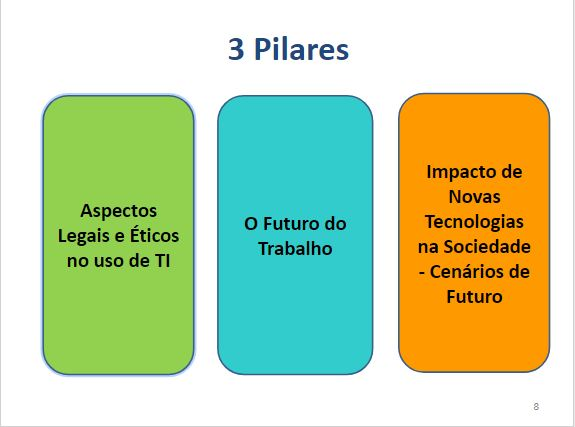
\includegraphics[scale=0.4]{Try.jpg}
     \caption{"Os pilares da cadeira de Informática e Sociedade em 2019.2."}
     \label{fig:imagem1}
\end{figure}



\section{Relevância}
\paragraph{}Esta cadeira é de suma importância para as pessoas do curso pois nela veremos coisas como:\newline
\textbf{Desenvolver um senso crítico:} Ela lhe ajudará nesse quesito a ter um ponto de vista mais fincado nos fatos, onde poderemos fazer projetos com os pés no chão, mas mesmo assim, mirando o desenvolvimento.\newline\newpage
\textbf{Se manter atualizado:} Nela aprendemos que temos que estar em constante aprendizado, e para isso, as professoras e monitores nos mantém atualizados com sites onde podemos encontrar esses fatos e onde podemos também achar fonte de pesquisas, como por exmeplo esse site onde ele fala sobre o uso do algoritmo do youtube.\cite{Site}
\begin{figure}[!htb]
     \centering
     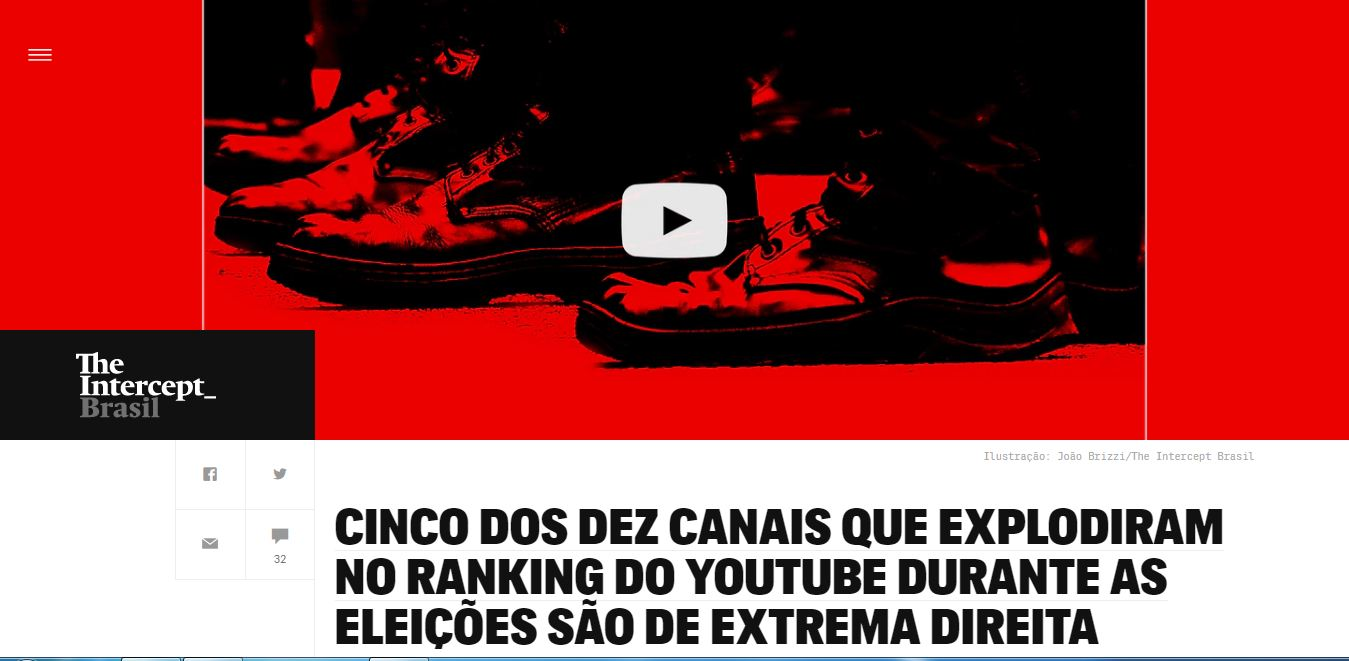
\includegraphics[scale=0.2]{Site.jpg}
     \caption{"Nesse artigo ele fala como o algoritmo do youtube tem efeitos sobre as eleições."}
     \label{fig:imagem1}
\end{figure}
\newline\textbf{A cooperação e trabalho em grupo:} Além de tudo isso que já foi mencionado, esta cadeira tem seu maior destaque em como ela estimula o trabalho em grupo, sempre visando com que o aluno perca a timidez de socializar e tirando ele da zona de conforto, ela se baseia em trabalhos e dinâmicas que todos tem que participar para receberem a nota.\cite{Site2}



\section{Relação com outras disciplinas}

\begin{table}[h]
    \caption{Tabela de relação}
    \centering
    \begin{tabular}{| l | l |}
         \hline
         Disciplina & Relaçãos \\
        \hline
        IF801 - Tecnologias Educacionais. & -Comunicação  e trabalho em grupo\\& \\\hline
        IF681 - Interface Usuário-Máquina. & -Servirá para construir a aproximação \\&entre humano e máquina na sociedade. \\\hline
        IF779 - Nova economia e nova sociedade. & -Como reduzir o impacto negativo \\&de novas tecnologias.\\\hline
    \end{tabular}
    \label{tab:my_label}
\end{table}


\bibliographystyle{plain}
\bibliography{lvs2}
\end{document}

